\documentclass{beamer}
\usetheme{Warsaw}
\useinnertheme{circles}
\useoutertheme[subsection=false]{smoothbars}
\usepackage[utf8x]{inputenc}
\usepackage[czech]{babel}
\usepackage[T1]{fontenc}
\usepackage{listings}
\usepackage{tikz}
\lstset{basicstyle=\tiny\ttfamily}
\logo{
\includegraphics[height=0.5cm]{brmlab.pdf}}

\begin{document}

\AtBeginSection[]
{
  \begin{frame}
    \frametitle{Outline}
    \tableofcontents[currentsection]
  \end{frame}
}

\title{brmiversity: Umělá inteligence \\ a teoretická informatika}
\subtitle{Přednáška č. 8}
\author{Petr Baudiš $\langle${\tt pasky@ucw.cz}$\rangle$}
\institute{
	brmlab 2011\\
	\vskip 1ex
	\pgfdeclareimage[height=4ex]{ccbysa}{by-sa.pdf}
	\pgfuseimage{ccbysa}
}
\date{}
\frame{\titlepage}

\section{Adaptivní agenti}

\subsection{}
\begin{frame}{Metody pro řízení agentů}
\begin{itemize}
\item BDI, SOAR, atd.
\end{itemize}
\end{frame}

\subsection{}
\begin{frame}{Otázky?}
\begin{center}
Příště: Metody pro učení agentů.
\end{center}
\end{frame}

\section{Neuronové sítě}

\subsection{}
\begin{frame}{ANN Revisited}
\begin{itemize}
\item Umělé neurony (``výpočetní krabičky'') \\ dostávají vstupy (čísla) a na jejich \\ základě generují výstup (číslo)
\item Obvykle: Vrstvy striktně oddělené, \\ vstupní vrstva se vstupy zvnějšku, \\ výstupní vrstva s výstupem pro uživatele, \\ skryté vrstvy vyhodnocují různé charakteristiky vstupů
\item Dnes: Více vrstev neuronů, jak je učit?
\end{itemize}
\begin{tikzpicture}[remember picture,overlay]
  \node [xshift=-4.5cm,yshift=-6cm,above right] at (current page.north east)
    {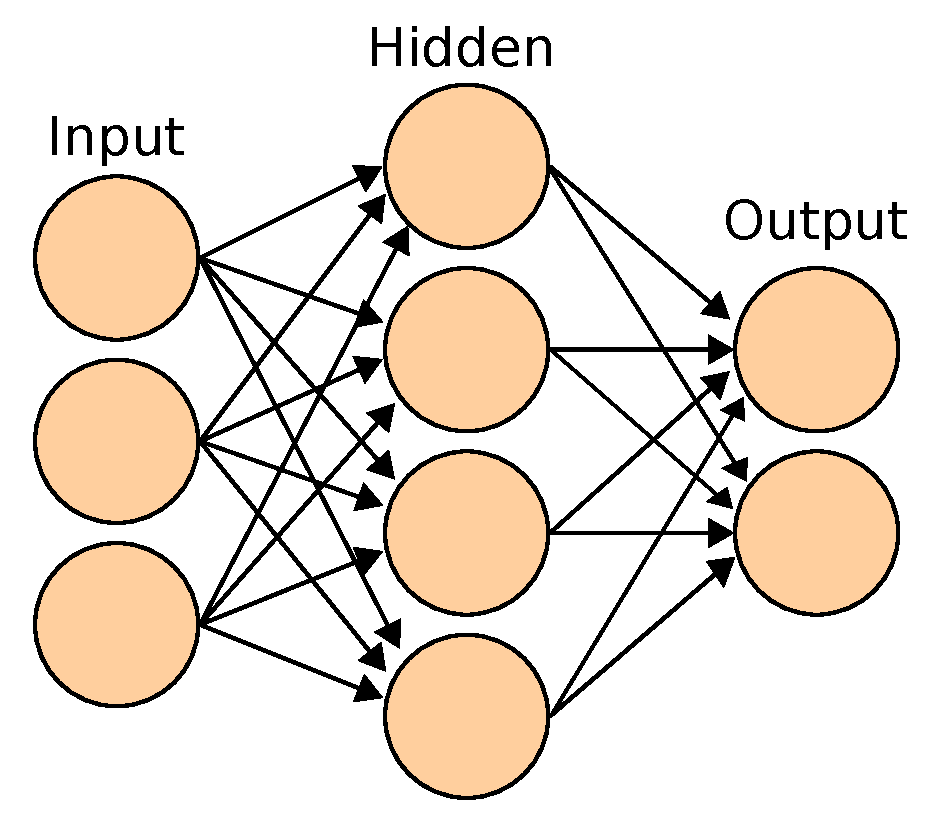
\includegraphics[width=4cm]{ANN.pdf}};
\end{tikzpicture}
\end{itemize}
\end{frame}

\subsection{}
\begin{frame}{Backpropagation Revisited}
\begin{itemize}
\item Myšlenka: Závislosti mezi vstupy a výstupy dokážeme přiměřeně matematicky popsat
\item Chceme upravit váhy podle {\em chyby}, kterou propagovaly; \\ větší váha nese větší chybu
\vskip 3ex
\item Iterujeme učení podle vstupních množin:
\begin{itemize}
\item Zjistíme chybu výstupu
\item Spočítáme {\em gradient} chyby podle vah jednotlivých spojů
\item Chybu se pokusíme zredukovat posunutím vah proti gradientu
\item Chybu ``zpětně šíříme'' do předchozí vrstvy a opakujeme
\end{itemize}
\end{itemize}
\end{frame}

\subsection{}
\begin{frame}{Vylepšení zpětného šíření}
\begin{itemize}
\item Gradienty, metody prvního a druhého řádu
\item Genetické algoritmy
\end{itemize}
\end{frame}

\subsection{}
\begin{frame}{Interní reprezentace znalostí}
\begin{itemize}
\item Prořezávání atd.
\end{itemize}
\end{frame}

\subsection{}
\begin{frame}{Otázky?}
\begin{center}
Příště: ANN úplně jinak --- asociativní paměti.
\end{center}
\end{frame}

\section{Složitost}

\subsection{}
\begin{frame}{Třídy složitosti}
\begin{itemize}
\item Rekapitulace --- P, NP, PSPACE, EXPTIME
\end{itemize}
\end{frame}

\subsection{}
\begin{frame}{Míry složitosti}
\begin{itemize}
\item Polynomiální hierarchie
\end{itemize}
\end{frame}

\subsection{}
\begin{frame}{Savičova věta}
\begin{itemize}
\item TODO
\end{itemize}
\end{frame}

\subsection{}
\begin{frame}{Konstruovatelné funkce}
\begin{itemize}
\item TODO
\end{itemize}
\end{frame}

\subsection{}
\begin{frame}{Otázky?}
\begin{center}
Příště: Technické důsledky tříd složitosti.
\end{center}
\end{frame}

\section{Vyčíslitelnost}

\subsection{}
\begin{frame}{Věty o rekurzi}
\begin{itemize}
\item Prvá, druhá, třetí, divná\dots
\end{itemize}
\end{frame}

\subsection{}
\begin{frame}{TODO jaxetojmenuje}
\begin{itemize}
\item Nelze určit, zda dva programy dělají to samé
\item Důkaz
\end{itemize}
\end{frame}

\subsection{}
\begin{frame}{Otázky?}
\begin{center}
Příště: Algoritmicky nerozhodnutelné problémy.
\end{center}
\end{frame}

\subsection{}
\begin{frame}{Děkuji vám}
\begin{center}
{\bf pasky@ucw.cz}

\vskip 6ex

Příště: Umělá inteligence (strojové učení).
	Neuronové sítě. \\
	Evoluční algoritmy (schémata, EP, GP). \\
	Datové struktury (binární vyhledávací stromy).
\end{center}
\end{frame}

\end{document}
